\chapter{Experimental Evaluation}
\label{sec:testing}

In this chapter, the experiments are described and analyzed. First, the B*-Tree placer performance is evaluated. Then, the test with various action sequence lengths is described. After that, results from the common benchmarks are evaluated and the proposed algorithm is compared with other state-of-the-art algorithms, including the previous work by the author \cite{vh}, which uses the similar approach but different representation (slicing tree). Finally, the conclusions are made.

\section{Placer Performance}

The speed of the B*-Tree placer was evaluated. The role of the placer is to process the given B*-Tree and to compute the exact position of each module based on the given tree structure. The exact process is mentioned in previous chapters. 

Several B*-Trees with increasing size were tested. Each tree was complete and balanced (except the leaves). The Table~\ref{tab:placer} shows the dependency of the placement time on the module count, including some basic distribution parameters (average, median, the standard population deviation and the time coefficient with the base / previous). The number of repeated runs was 10,000.

The conclusion is that twice as many modules take about 2.5 times more time to place. The measured time complexity seems to be close to linear ($O(n)$) for a reasonable amount of modules (to 10,000).

\begin{table}
\centering
\begin{tabular}{|c|c|c|c|c|}
\hline
Modules & Average [ms] & Median [ms] & Deviation [ms] & Coeficient [--] \\ 
\hline
\hline
100 & 0.057 & 0 & 0.398 & 1/1 (base) \\
\hline
200 & 0.111 & 0 & 0.423 & 1.947/1.947 \\
\hline
400 & 0.25 & 0 & 0.531 & 4.386/2.252 \\
\hline
800 & 0.635 & 1 & 0.816 & 11.14/2.54 \\
\hline
1,600 & 1.535 & 1 & 1.48 & 26.93/2.417 \\
\hline
3,200 & 4.063 & 4 & 2.769 & 71.28/2.647 \\ 
\hline
6,400 & 11.085 & 11 & 2.852 & 194.473/2.728 \\
\hline
12,800 & 34.582 & 34 & 4.905 & 606.701/3.12 \\
\hline
25,600 & 92.987 & 93 & 8.361 & 1,631.35/2.689 \\
\hline
\end{tabular}
\caption{Performance of the B*-Tree placer}
\label{tab:placer}
\end{table}

\section{Action Sequence Length}

Another experiment was prepared to evaluate how the action sequence length influences the solution quality. The length of the action sequence varies from 1 to 5 actions, the rest of the parameters was set as follows: $ I=1000, G=200, S=50 $. The results obtained are shown in the Table~\ref{tab:length}. The value shown is the unused area of the best result, averaged from 3 runs. The results show that the best length for action sequences for evaluated benchmarks is 3. Of course, this number can be different for various benchmarks.

\begin{table}
\centering
\begin{tabular}{|r|c|c|c|c|c|}
\hline
Test & $L=1$ & $L=2$ & $L=3$ & $L=4$ & $L=5$ \\
\hline
\hline
ami33 & 66395 & 66297 & 49588 & 65742 & 54897 \\
\hline
ami49 & 1988224 & 1846190 & 1480388 & 1596551 & 1811432 \\
\hline
n100 & 12952 & 13060 & 10501 & 11322 & 14323 \\
\hline
n200 & 19600 & 16330 & 15854 & 16585 & 16157 \\
\hline
\end{tabular}
\caption{Action sequence length and its influence on the performace}
\label{tab:length}
\end{table}

\section{Action Distribution}

For two benchmarks, {\em n300} and {\em ami49}, the population action type distribution was examined. Three statistics were counted for each action type: the total action creation count, the same count in the last generation and in the best solutions. All three numbers are sums for all iterations. The results are shown in Fig.~\ref{fig:statn300} (for {\em n300}) and Fig.~\ref{fig:statami49} (for {\em ami49}). The algorithm setup (the population size, the number of iterations, etc.) was the same for both tests.

It seems that the more modules the benchmark contains, the bigger amount of disabled actions (nop) are in the population. This can prove a theory that enabled actions are more `dangerous' to the prototype and mostly decrease its quality. As the amount of disabled actions grows over time, it seems that the algorithm tends to  fine-tune the prototype (`do less but better') before the optimisation ends.

\begin{figure}[p]
\centering
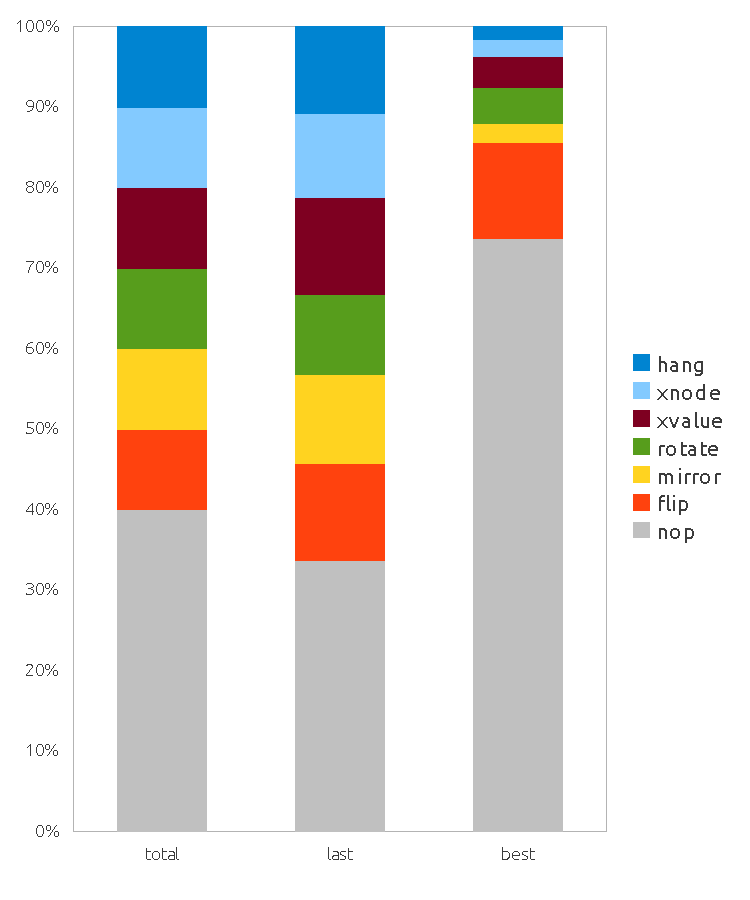
\includegraphics[width=\textwidth]{statn300}
\caption{The action distribution in {\em n300} (total, last generations, best solutions)}
\label{fig:statn300}
\end{figure}

\begin{figure}[p]
\centering
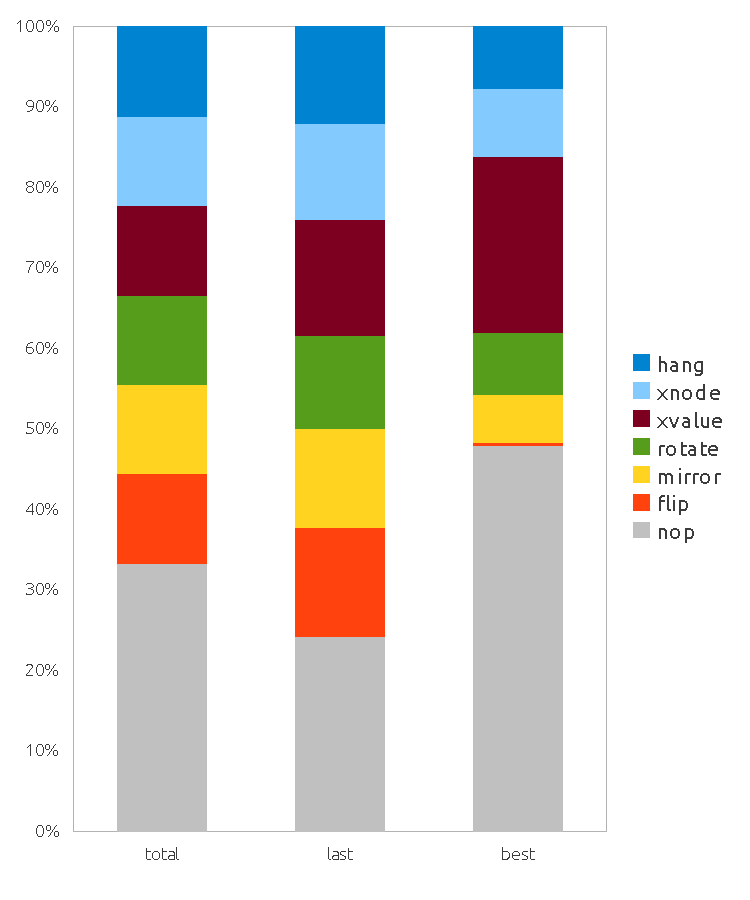
\includegraphics[width=\textwidth]{statami49}
\caption{The action distribution in {\em ami49} (total, last generations, best solutions)}
\label{fig:statami49}
\end{figure}

\section{GSRC Benchmarks}

Three benchmarks ({\em n100}, {\em n200}, {\em n300}) were selected from GSRC \cite{benchgsrc} and tested. The results are shown in Table~\ref{tab:gsrc}. Various algorithm setup parameters were evaluated. In the table, setup parameters with the resulting unused area statistics (average, the standard population deviation) and the computation time are displayed. The test indicate that the longer (in the terms of iterations) is the algorithm executed, the higher quality of the result can be achieved.

\begin{table}
\centering
\begin{tabular}{|r|c|c|c|c|c|c|c|}
\hline
Test & I & G & N & S & Unused area (avg) & Unused area (stdevp) & Time [ms] \\
\hline
\hline
n100 & 1000 & 1000 & 3 & 50 & 9443 & 1212 & 131716 \\
n100 & 2000 & 1000 & 3 & 50 & 8596 & 1103 & 306331 \\
n100 & 5000 & 1000 & 3 & 50 & 7488 & 1045 & 769864 \\
n100 & 10000 & 1000 & 3 & 50 & 5761 & 700 & 1575026 \\
n100 & 20000 & 1000 & 3 & 50 & 5254 & 330 & 3145128 \\
\hline
n200 & 1000 & 1000 & 3 & 50 & 14397 & 936 & 248533 \\
n200 & 2000 & 1000 & 3 & 50 & 12098 & 937 & 552172 \\
n200 & 5000 & 1000 & 3 & 50 & 9518 & 326 & 1405009 \\
n200 & 10000 & 1000 & 3 & 50 & 8136 & 760 & 3041565 \\
n200 & 20000 & 1000 & 3 & 50 & 7590 & 328 & 6067438 \\
\hline
n300 & 1000 & 1000 & 3 & 50 & 23167 & 2007 & 387434 \\
n300 & 2000 & 1000 & 3 & 50 & 19997 & 1784 & 862327 \\
n300 & 5000 & 1000 & 3 & 50 & 17156 & 1442 & 2163184 \\
n300 & 10000 & 1000 & 3 & 50 & 14645 & 1137 & 4690839 \\
n300 & 20000 & 1000 & 3 & 50 & 12929 & 494 & 9199609 \\
\hline
\end{tabular}
\caption{The GSRC benchmark results (10 runs)}
\label{tab:gsrc}
\end{table}

\begin{figure}
\centering
\subfloat[n100 (2.0\% dead)]{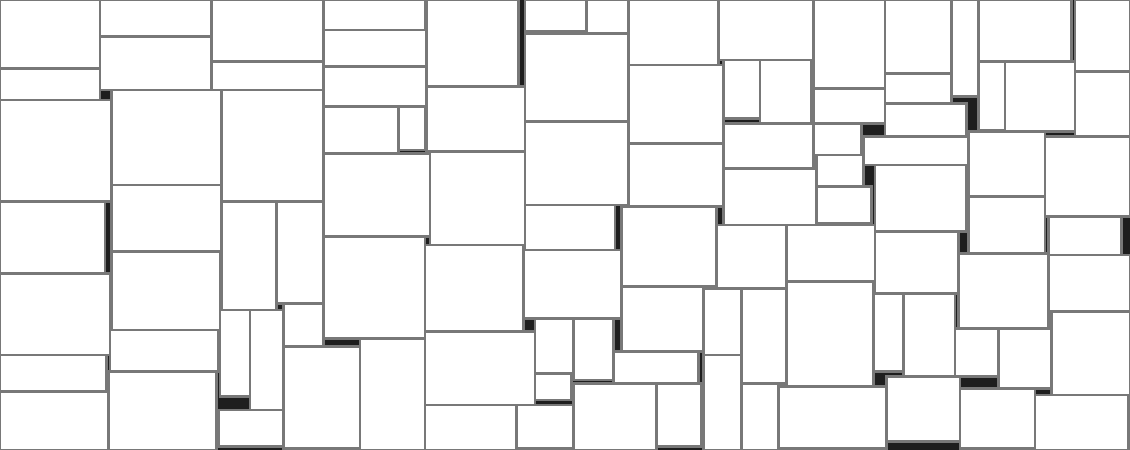
\includegraphics[height=3.9cm]{n100a}} \hfill
\subfloat[n100 (2.6\% dead)]{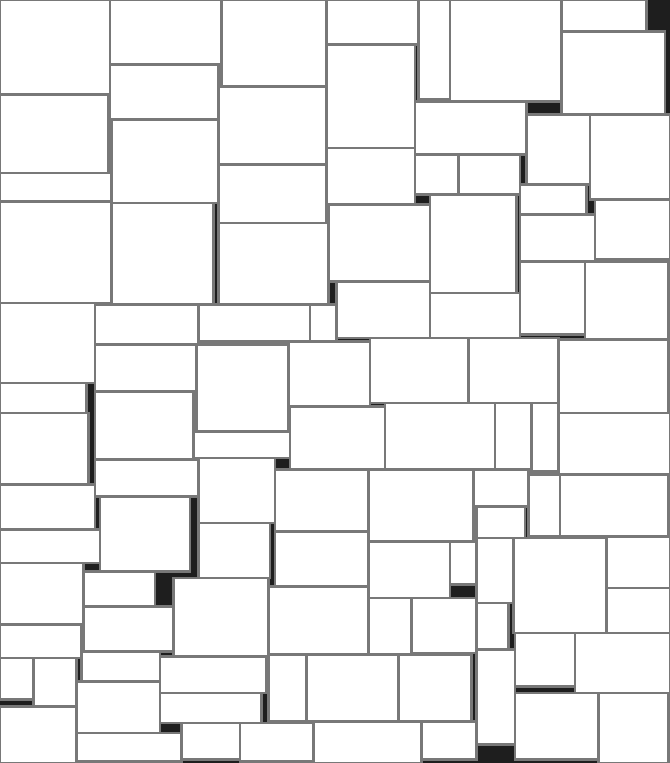
\includegraphics[angle=90,height=3.9cm]{n100b}} \\
\subfloat[n200 (3.4\% dead)]{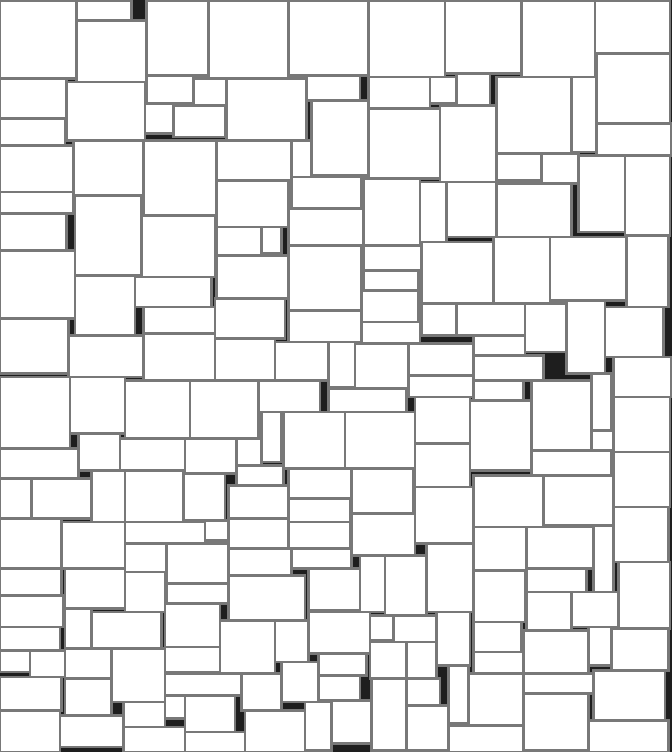
\includegraphics[angle=90,height=6.1cm]{n200a}} \hfill
\subfloat[n200 (4.1\% dead)]{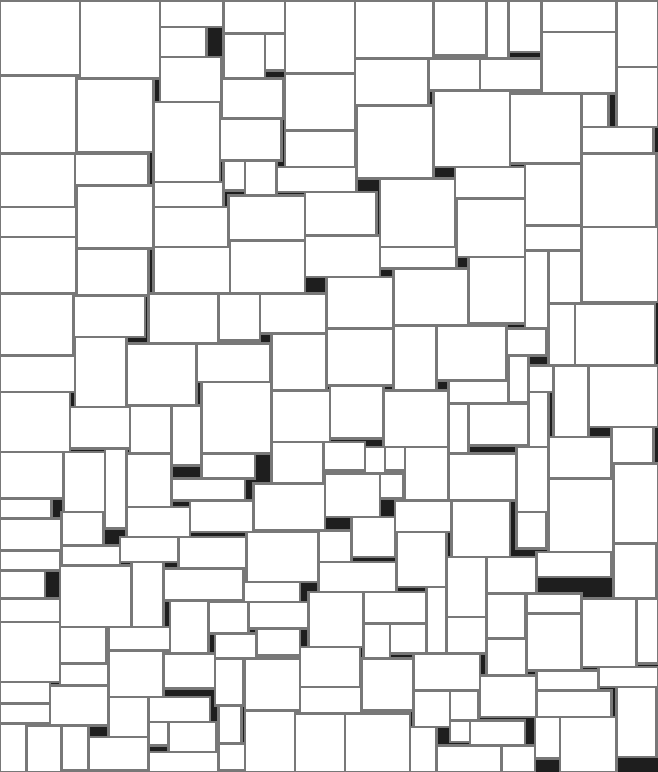
\includegraphics[angle=90,height=6.1cm]{n200b}} \\
\subfloat[n300 (3.8\% dead)]{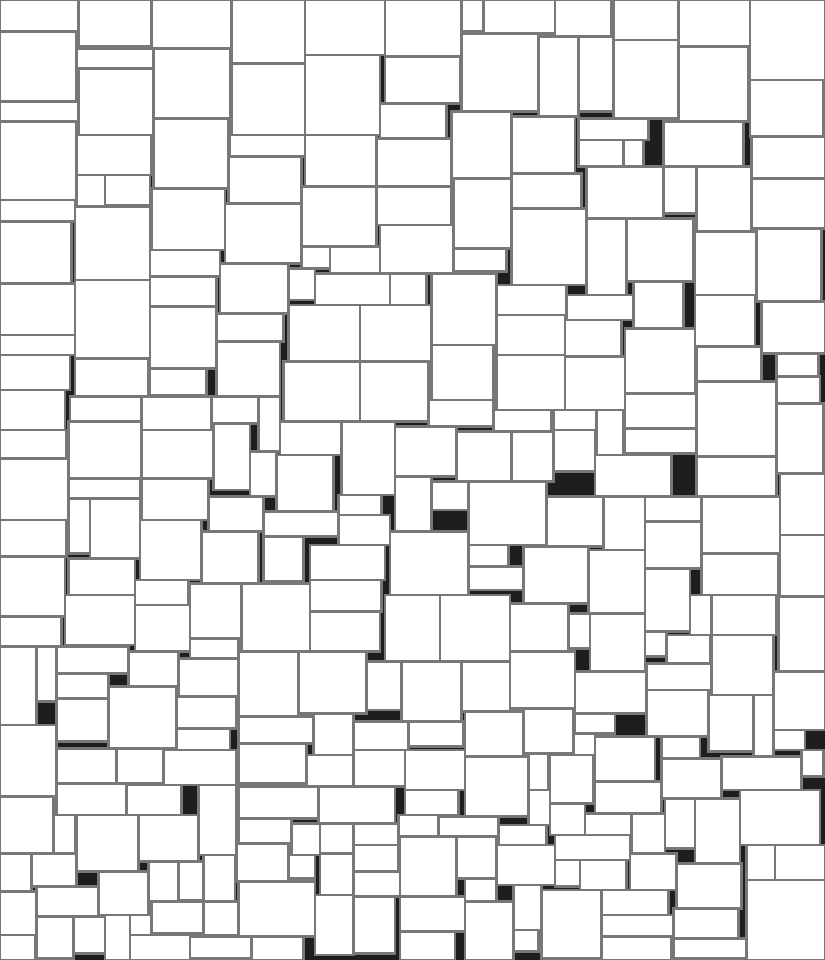
\includegraphics[angle=90,height=6.1cm]{n300a}} \hfill
\subfloat[n300 (4.6\% dead)]{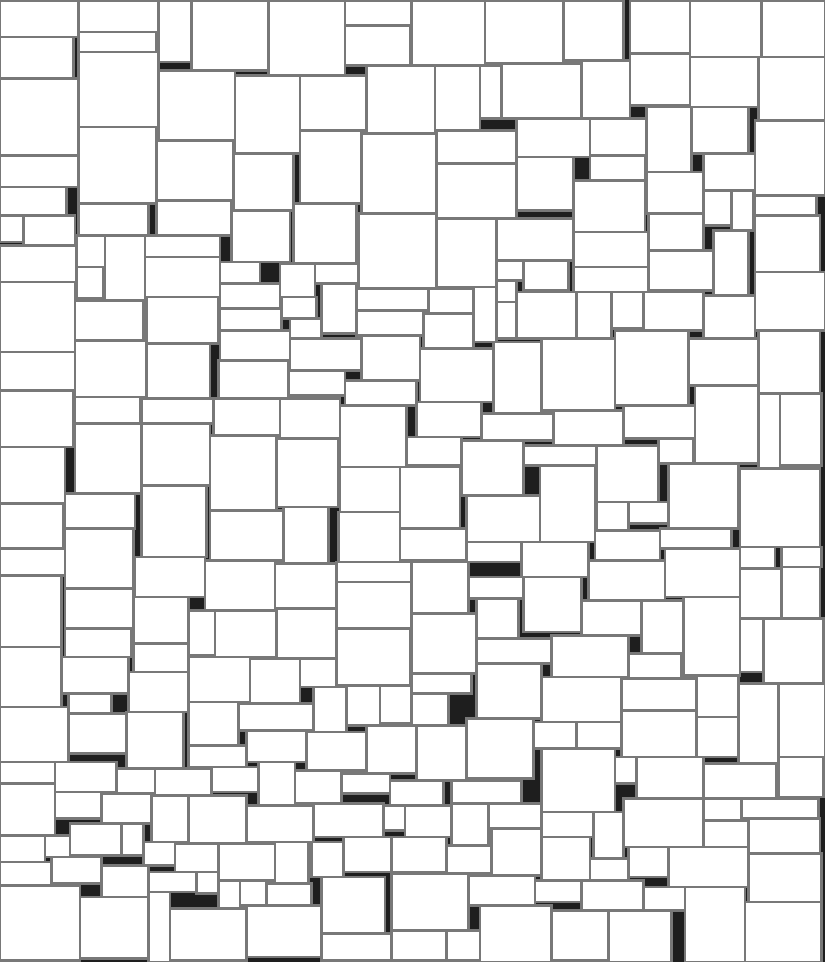
\includegraphics[angle=90,height=6.1cm]{n300b}} \\
\caption{The best solutions of GSRC benchmarks found}
\label{fig:gsrc}
\end{figure}

\section{MCNC Benchmarks}

Five benchmarks ({\em ami33}, {\em ami49}, {\em apte}, {\em hp}, {\em xerox}) were selected from MCNC \cite{benchmcnc} and tested. The results are shown in Table~\ref{tab:mcnc}. Various algorithm setup parameters were evaluated. The table has the same structure as the Table~\ref{tab:gsrc}. The algorithm performance trend is the same as for GSRC benchmarks.

\begin{table}
\centering
\begin{tabular}{|r|c|c|c|c|c|c|c|}
\hline
Test & I & G & N & S & Unused area (avg) & Unused area (stdevp) & Time [ms] \\
\hline
\hline
ami33 & 1000 & 1000 & 3 & 50 & 51038 & 12382 & 57231 \\
ami33 & 2000 & 1000 & 3 & 50 & 43448 & 7939 & 125401 \\
ami33 & 5000 & 1000 & 3 & 50 & 35858 & 6512 & 308969 \\
ami33 & 10000 & 1000 & 3 & 50 & 28503 & 7720 & 654963 \\
ami33 & 20000 & 1000 & 3 & 50 & 26445 & 7330 & 1276712 \\
\hline
ami49 & 1000 & 1000 & 3 & 50 & 1535562 & 300083 & 73698 \\
ami49 & 2000 & 1000 & 3 & 50 & 1220844 & 227792 & 166745 \\
ami49 & 5000 & 1000 & 3 & 50 & 1025001 & 149170 & 413727 \\
ami49 & 10000 & 1000 & 3 & 50 & 964594 & 83946 & 871935 \\
ami49 & 20000 & 1000 & 3 & 50 & 906892 & 140213 & 1698927 \\
\hline
apte & 1000 & 1000 & 3 & 50 & 363220 & 0 & 35993 \\
apte & 2000 & 1000 & 3 & 50 & 363220 & 0 & 76266 \\
apte & 5000 & 1000 & 3 & 50 & 363220 & 0 & 185827 \\
apte & 10000 & 1000 & 3 & 50 & 363220 & 0 & 379578 \\
apte & 20000 & 1000 & 3 & 50 & 363220 & 0 & 771397 \\
\hline
hp & 1000 & 1000 & 3 & 50 & 497565 & 63731 & 36817 \\
hp & 2000 & 1000 & 3 & 50 & 491979 & 69373 & 79436 \\
hp & 5000 & 1000 & 3 & 50 & 407131 & 130635 & 193348 \\
hp & 10000 & 1000 & 3 & 50 & 378495 & 142483 & 401036 \\
hp & 20000 & 1000 & 3 & 50 & 276830 & 138655 & 800229 \\
\hline
xerox & 1000 & 1000 & 3 & 50 & 615342 & 84494 & 33845 \\
xerox & 2000 & 1000 & 3 & 50 & 579978 & 76779 & 71782 \\
xerox & 5000 & 1000 & 3 & 50 & 567126 & 93078 & 174733 \\
xerox & 10000 & 1000 & 3 & 50 & 578195 & 104389 & 361800 \\
xerox & 20000 & 1000 & 3 & 50 & 536545 & 73416 & 723015 \\
\hline
\end{tabular}
\caption{The MCNC benchmark results (10 runs)}
\label{tab:mcnc}
\end{table}

\begin{figure}
\centering
\subfloat[apte (0.8\% dead)]{
\includegraphics[width=\textwidth]{apte}} \\
\subfloat[hp (3.9\% dead)]{
\includegraphics[angle=90,width=\textwidth]{hp}} \\
\subfloat[ami33 (1.6\% dead)]{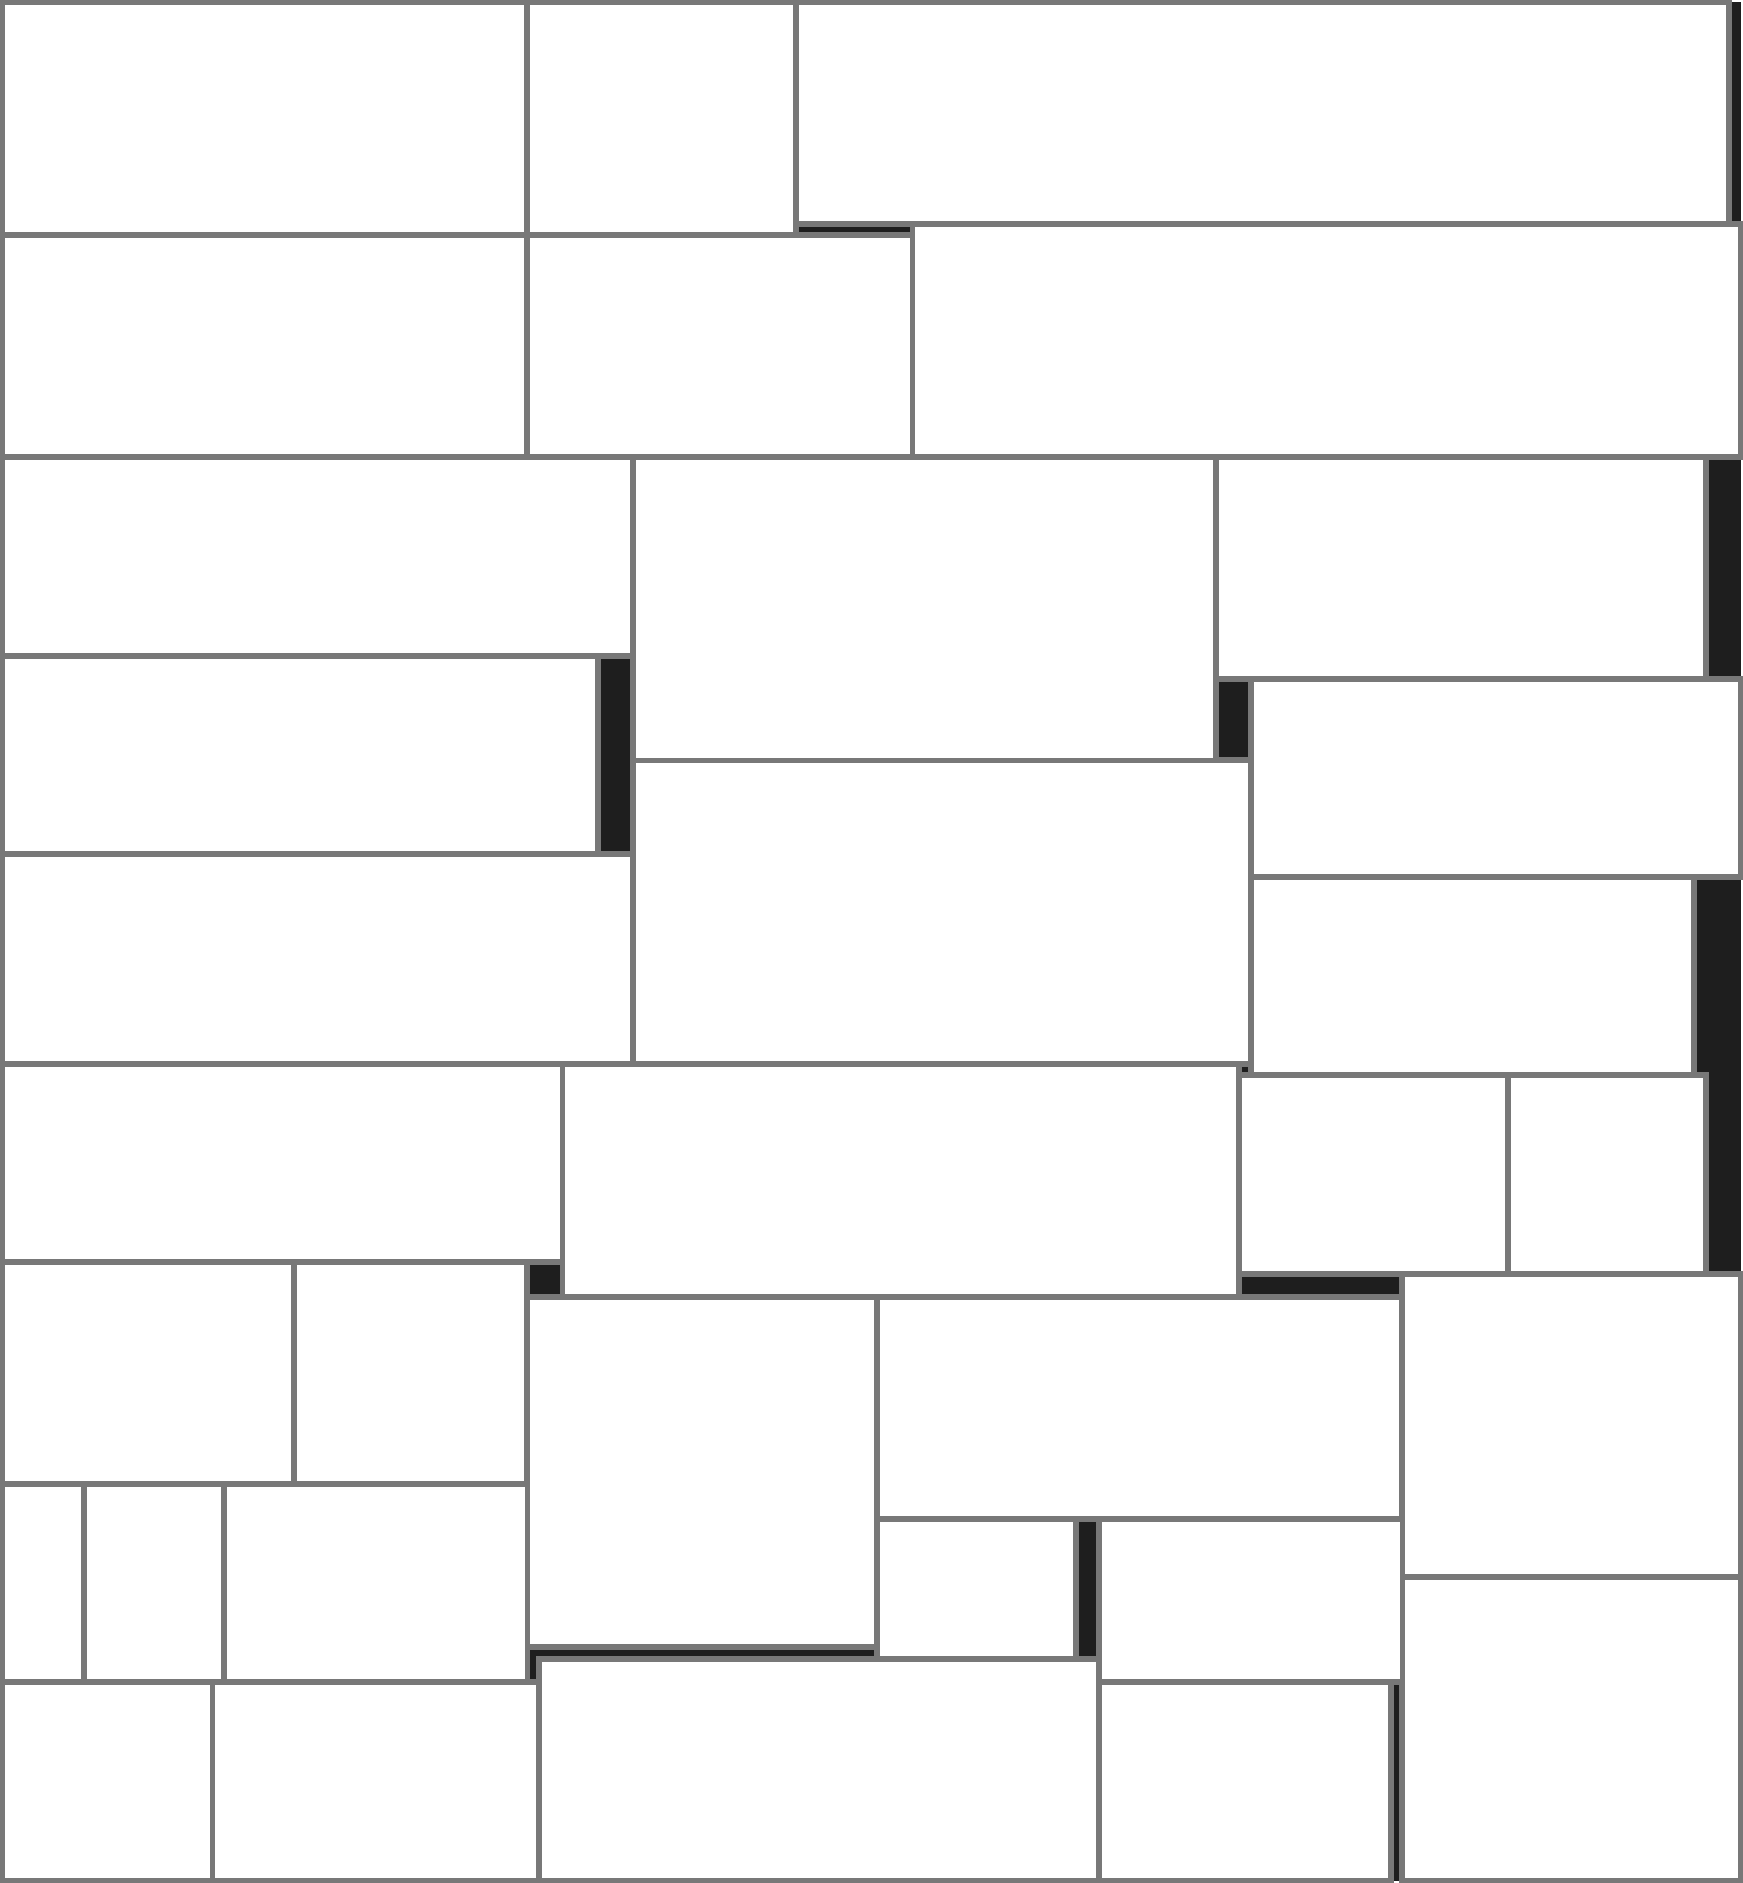
\includegraphics[angle=90,width=.47\textwidth]{ami33}} \hfill
\subfloat[ami49 (2.1\% dead)]{\includegraphics[angle=90,width=.47\textwidth]{ami49}} \\
\subfloat[xerox (2.3\% dead)]{\includegraphics[width=.6\textwidth]{xerox}} \\
\caption{The best solutions of MCNC benchmarks found}
\label{fig:mcnc}
\end{figure}

\section{Comparsion with Recent Algorithms}

The algorithm implemented was compared with some of recent algorithms in the field and to the previous work by author \cite{vh}, which uses the same optimisation framework but different representation (slicing tree). Results of this comparsion are shown on Table~\ref{tab:bachelor}. Unfortunately, getting and comparing the results is hard, because every article uses different benchmarks and watches different floorplan measures (e.g. total area instead of unused area). Also the time is given for rough estimation only, as the tests were performed on different machines. Our configuration was run at 2~GHz CPU. Results are shown on Table~\ref{tab:stateofart}. Both short run ($I=2000,G=1000$) and long run ($I=50000,G=1000$) of the algorithm are shown.

\begin{table}
\centering
\begin{tabular}{|r|c|c|c|c|}
\hline
Test & \multicolumn{2}{|c|}{POEMS/Slicing (unused area, time)} & \multicolumn{2}{|c|}{POEMS/B*-Tree (unused area, time)} \\
\hline
\hline
n100 & {\bf 11,142} & 3,741,504 ms & {\bf 5,761} & 1,575,026 ms \\
\hline
n200 & {\bf 17,636} & 8,500,771 ms & {\bf 8,136} & 3,041,565 ms \\
\hline
\end{tabular}
\caption{Comparsion with the previous work}
\label{tab:bachelor}
\end{table}

\begin{table}
\centering
\begin{tabular}{|r|c|c|c|c|c|}
\hline
 & \multicolumn{2}{|c|}{POEMS/B*-Tree} & CompaSS & B*-Tree & B*-Tree/SA \\
\hline
Test & long run & short run & see \cite{bench} & see \cite{btree} & see \cite{btreesa} \\
\hline
\hline
apte & 0.78\% (969 s) & 0.78\% (76 s) & 0.78\% (0 s) & {\bf 0.77\%} (7 s) & 1.59\% (2 s) \\
\hline
xerox & {\bf 2.30\%} (902 s) & 3.00\% (71 s) & 3.45\% (16 s) & 2.48\% (25 s) & 3.85\% (5 s) \\
\hline
hp & 3.88\% (1,927 s) & 5.57\% (79 s) & 2.28\% (3 s) & {\bf 1.35\%} (55 s) & 4.47\% (20 s) \\
\hline
n100 & {\bf 1.98\%} (4,826 s) & 4.79\% (306 s) & 7.32\% (4 s) & N/A & N/A \\
\hline
n200 & {\bf 3.68\%} (8,408 s) & 6.89\% (552 s) & 6.48\% (10 s) & N/A & N/A \\
\hline
\end{tabular}
\caption{Comparsion with recent algorithms}
\label{tab:stateofart}
\end{table}

\clearpage
\section{Conclusions}
\label{sec:conclusions}

\subsection{Outcomes}

A brand new solver for the 2D rectangle packing problem (floorplanning) was designed, implemented and tested. It is based on the POEMS iterative optimisation framework and genetic algorithm, used for local search. The best-fit inspired heuristic was used in order to create the prototype solution of each problem and 6 different actions for modifying it. 

The algorithm was implemented in the Java programming language version 1.6 and tested on public benchmark data available on the website \cite{bench} (GSRC \cite{benchgsrc}, MCNC \cite{benchmcnc}). The results were compared to the author's previous work \cite{vh} and to some of the state-of-the-art algorithms. It was very difficult to compare all algorithms as most of them have multiple setup parameters that significantly influence the solution quality and the computation time.

The experiments show that the suggested algorithm is competetive in quality, and even slightly better than all the other algorithms tested. Its performance is strongly dependent on the iteration and generation count, so the timing constraints must be taken into account. If the result quality is critical and the computation time not limited, the proposed algorithm is a good choice. It outperforms CompaSS \cite{bench} and B*-Tree/SA \cite{btreesa} in all benchmarks. Usually, in about 1 hour, satisfactory to very good results are acquired. If the result quality is not crucial, a setup running for several minutes can be sufficient for solving smaller problem instances.

The new algorithm was also compared to the previous work by the author \cite{vh}. The best results from the previous work and the second best results were taken from the current implementation (as the time magnitude is similar). For both benchmarks, the performance of the new algorithm is roughly twice as good and the result was obtained twice as fast.

\subsection{Further Work}

Further development of the algorithm could include dealing with pre-placed or soft modules. Another advantage of the B*-Tree is that it can be quite easily extended to work with rectilinear modules (for instance, T-shaped or L-shaped modules). That can be done by splitting these rectilinear shapes into rectangles and modifying the placing algorithm to keep those corresponding rectangles compacted. Several articles that work with this solution have already been published.

Another extension possibility is to add support for placing and optimising soft modules. This change can be implemented, for example, by adding a `ratio' parameter to each B*-Tree node, which is optimised too. This parameter is kept to stay in the range specified by the problem assignement (usually, the problems specify the minimum and the maximum ratio allowed for each module).

Finally, the most versatile floorplan optimiser would support both of these extensions mentioned above. The combination is not simple, as it is difficult to specify the ratio range of a general rectilinear module (the problem is to specify the meaning of the `ratio' itself).

Optimisation of the wirelength is easy to add, too. A different loading procedure for the input data must be implemented and the fitness function calculation must be changed, and that is all. And, perhaps, the function for creating of a prototype could be also changed to take interconnection into account.
